\documentclass[tikz]{standalone} % El secreto está aquí
\usetikzlibrary{shapes, arrows, positioning, calc}

\begin{document}
	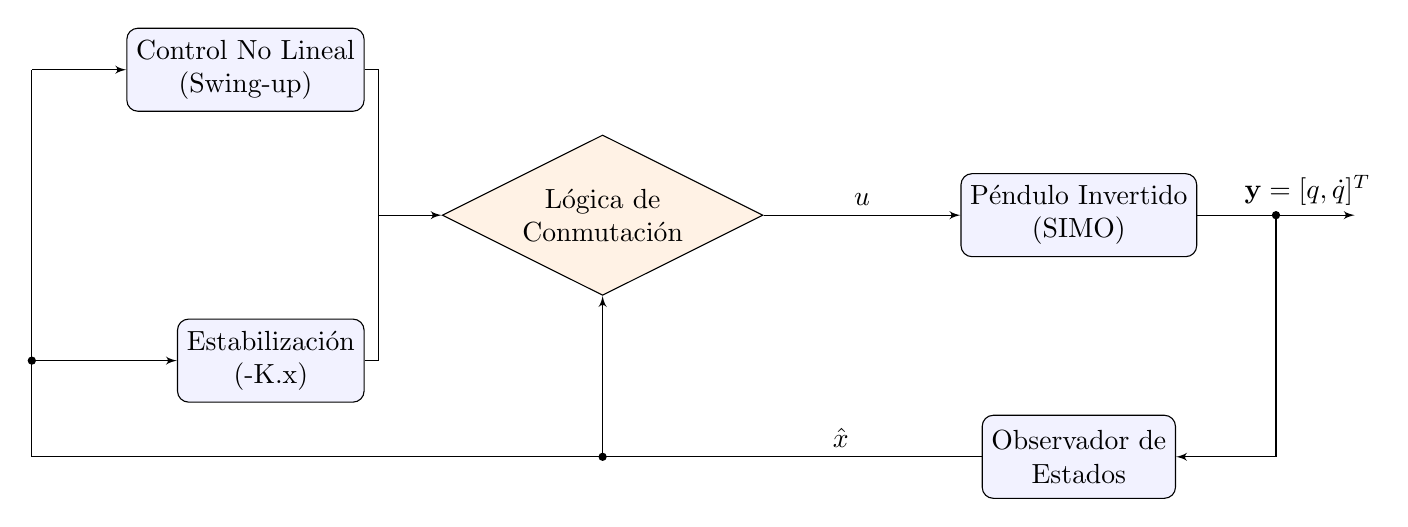
\begin{tikzpicture}[auto, node distance=2.5cm, >=latex']
    \tikzset{
		block/.style={draw, fill=blue!5, rectangle, minimum height=3em, minimum width=6em, align=center, rounded corners},
		logic/.style={draw, fill=orange!10, diamond, aspect=2, minimum width=4em, align=center},
		sum/.style={draw, circle, node distance=1cm},
		input/.style={coordinate},
		output/.style={coordinate}
	}
	        % --- Nivel de Decisión ---
	\node [logic] (logic) {Lógica de\\ Conmutación};
	\node [block, above left=0.8cm and 2cm of logic] (swing) {Control No Lineal\\ (Swing-up)};
	\node [block, below left=0.8cm and 2cm of logic] (stab) {Estabilización\\ (-K.x)};
	
	% --- Planta y Observador ---
	\node [block, right=2.5cm of logic] (plant) {Péndulo Invertido\\ (SIMO)};
	\node [block, below=2cm of plant] (obs) {Observador de\\ Estados};
	
	% --- Conexiones de Control a la Lógica ---
	% Creamos un punto de unión limpio antes de entrar al diamante
	\coordinate (join_c) at ($(logic.west) + (-0.8, 0)$);
	\draw (swing.east) -| (join_c);
	\draw (stab.east) -| (join_c);
	\draw [->] (join_c) -- (logic.west);
	
	% --- Conexión u de Lógica a Planta ---
	\draw [->] (logic.east) -- node[name=u, above] {$u$} (plant.west);
	% Guardamos el punto medio para sacar la señal al observador
	\coordinate (u_meas) at ($(logic.east)!0.5!(plant.west)$);
	
	% --- Salidas SIMO (1 a 2) ---
	\coordinate (y_out) at ($(plant.east) + (2, 0)$);
	\draw [->] (plant.east) -- node[pos=0.7, above] {$\mathbf{y} = [q, \dot{q}]^T$} (y_out);
	% Guardamos el punto de bifurcación de la salida
	\coordinate (y_meas) at ($(plant.east) + (1, 0)$);
	
	% --- Entradas al Observador ---
	\draw [->] (y_meas) |- (obs.east);
	
	% Dibujamos los puntos de conexión de y
	\fill (y_meas) circle (1.5pt);
	
	% --- Estado Estimado (Realimentación) ---
	% 1. Sacamos la señal por la izq del observador
	\coordinate (x_out) at ($(obs.west) + (0, 0)$);
	
	% 2. Calculamos el límite izquierdo (más a la izquierda que los controladores)
	\coordinate (x_left) at ($(swing.west) + (-1.2, 0)$);
	
	% 3. Dibujar las conexiones del estado estimado. 
	\draw (obs.west) -- (x_out) -| (x_left);
	
	% 4. Ramificación superior (Swing-up)
	\draw [->] (x_left) -- (swing.west);
	
	% 5. Ramificación media (Estabilización)
	\coordinate (x_stab) at (x_left |- stab.west);
	\draw [->] (x_stab) -- (stab.west);
	\fill (x_stab) circle (1.5pt); % Punto de conexión
	
	% 6. Ramificación hacia la Lógica de Conmutación 
	\coordinate (x_logic) at (x_out -| logic.south);
	\draw [->] (x_logic) -- node[right] {} (logic.south);
	\fill (x_logic) circle (1.5pt); % Punto de conexión
	
	% --- Etiqueta del estado estimado \hat{x} ---
	\path (x_out -| plant.south) -- node[above] {$\hat{x}$} (x_logic);	% ... nodos y conexiones ...
	\end{tikzpicture}
\end{document}